\usetikzlibrary{arrows.meta}
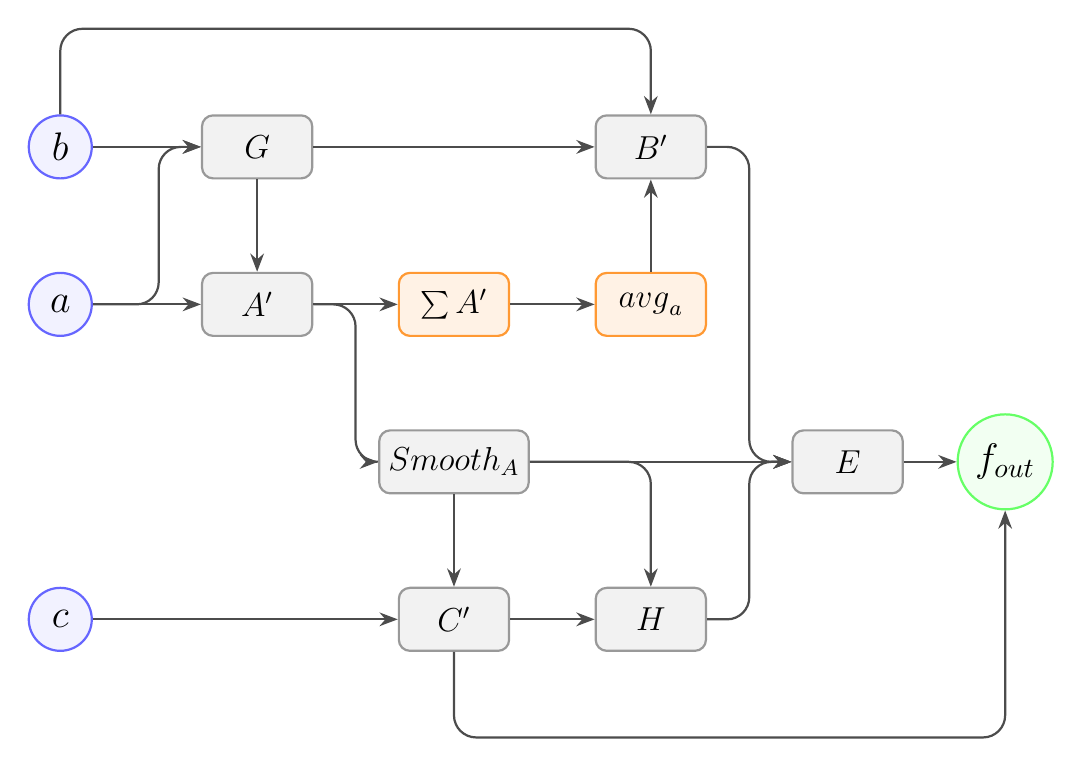
\begin{tikzpicture}[
    >=Stealth,
    % 统一定义节点样式
    input/.style={circle, draw=blue!60, fill=blue!5, thick, minimum size=8mm, font=\Large},
    output/.style={circle, draw=green!60, fill=green!5, thick, minimum size=8mm, font=\Large},
    op/.style={rectangle, draw=gray!80, fill=gray!10, thick, rounded corners, minimum width=1.4cm, minimum height=0.8cm, font=\large},
    global/.style={rectangle, draw=orange!80, fill=orange!10, thick, rounded corners, minimum width=1.4cm, minimum height=0.8cm, font=\large\bfseries},
    % 连线样式：加入 rounded corners=8pt 让正交拐角变得圆润、具有科技感
    edge/.style={->, thick, draw=black!70, rounded corners=8pt}
]

% ==================== 重新排列的绝对坐标网格 ====================

% 顶部计算流
\node[input] (b) at (0, 0) {$b$};
\node[op] (G) at (2.5, 0) {$G$};
\node[op] (Bprime) at (7.5, 0) {$B'$};

% 中上计算流 (同步层)
\node[input] (a) at (0, -2) {$a$};
\node[op] (Aprime) at (2.5, -2) {$A'$};
\node[global] (sum) at (5, -2) {$\sum A'$};
\node[global] (avg) at (7.5, -2) {$\text{avg}_a$};

% 中下计算流 (融合层)
\node[op] (Smooth) at (5, -4) {$\text{Smooth}_A$};
\node[op] (E) at (10, -4) {$E$};
\node[output] (out) at (12, -4) {$f_{\text{out}}$};

% 底部计算流
\node[input] (c) at (0, -6) {$c$};
\node[op] (Cprime) at (5, -6) {$C'$};
\node[op] (H) at (7.5, -6) {$H$};

% ==================== 智能正交连线 (零交叉) ====================

% 1. 到 G 和 A' 的基础输入 (左侧)
\draw[edge] (b) -- (G);
\draw[edge] (a) -- (Aprime);
\draw[edge] (a) -| (1.25, 0) -- (G); % a 到 G：向右半步，再向上，再平入
\draw[edge] (G) -- (Aprime);

% 2. 全局同步主线 (中间层)
\draw[edge] (Aprime) -- (sum);
\draw[edge] (sum) -- (avg);
\draw[edge] (avg) -- (Bprime);

% 3. 跨度较大的 B' 依赖 (避开下方节点)
\draw[edge] (G) -- (Bprime); % G 到 B'：平移，完美避让
\draw[edge] (b.north) |- (3.75, 1.5) -| (Bprime.north); % b 到 B'：从顶部上方绕行通道

% 4. Smooth_A 和 C' 的前置
\draw[edge] (Aprime) -| (3.75, -4) -- (Smooth); % A' 到 Smooth
\draw[edge] (c) -- (Cprime);
\draw[edge] (Smooth) -- (Cprime);

% 5. H 的计算
\draw[edge] (Cprime) -- (H);
\draw[edge] (Smooth) -| (H.north); % Smooth 到 H：向右合并后向下流入

% 6. E 的多路数据汇聚 (总线式合并)
\draw[edge] (Smooth) -- (E);
\draw[edge] (Bprime.east) -| (8.75, -4) -- (E); % 从上方降下，并入 -4 层总线
\draw[edge] (H.east) -| (8.75, -4) -- (E);      % 从下方升起，并入 -4 层总线

% 7. 最终输出
\draw[edge] (E) -- (out);
\draw[edge] (Cprime.south) |- (8.5, -7.5) -| (out.south); % C' 到 out：从底部下方绕行通道

\end{tikzpicture}